\subsection*{1. Política de escalonamento e prioridades}
\addcontentsline{toc}{section}{1. Política de escalonamento e prioridades}

\subsubsection{1.1 - Compile com a opção -pthread e execute o programa prog1.c. Veja as opções do programa e execute cada uma delas. É necessário ser usuário root para alguma delas.}
\addcontentsline{toc}{subsection}{Exercício 1.1}

\vspace{-0.5em}
\begin{minipage}{\textwidth}
  \hspace{1em}
  \centering
  \lstinputlisting[language=C, firstline=133, lastline = 171]{pratica2/prog1.c}
  \captionof{figure}{Trecho do código-fonte do prog1.c com opções de entrada}
  \label{prog1}
  \hspace{1em}
\end{minipage}
\vspace{0.5em}

\vspace{2em}
\begin{minipage}{\textwidth}
    \hspace{-1em}
    \centering
    \begin{minipage}[b]{0.32\textwidth}
        \centering
        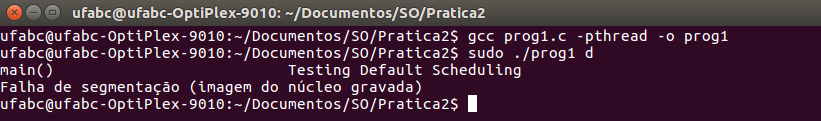
\includegraphics[trim=0 0 85 0,clip,scale=.25]{pratica2/prog1-d.png}
        
        (a)
    \end{minipage}
    \hfill
    \begin{minipage}[b]{0.32\textwidth}
        \centering
        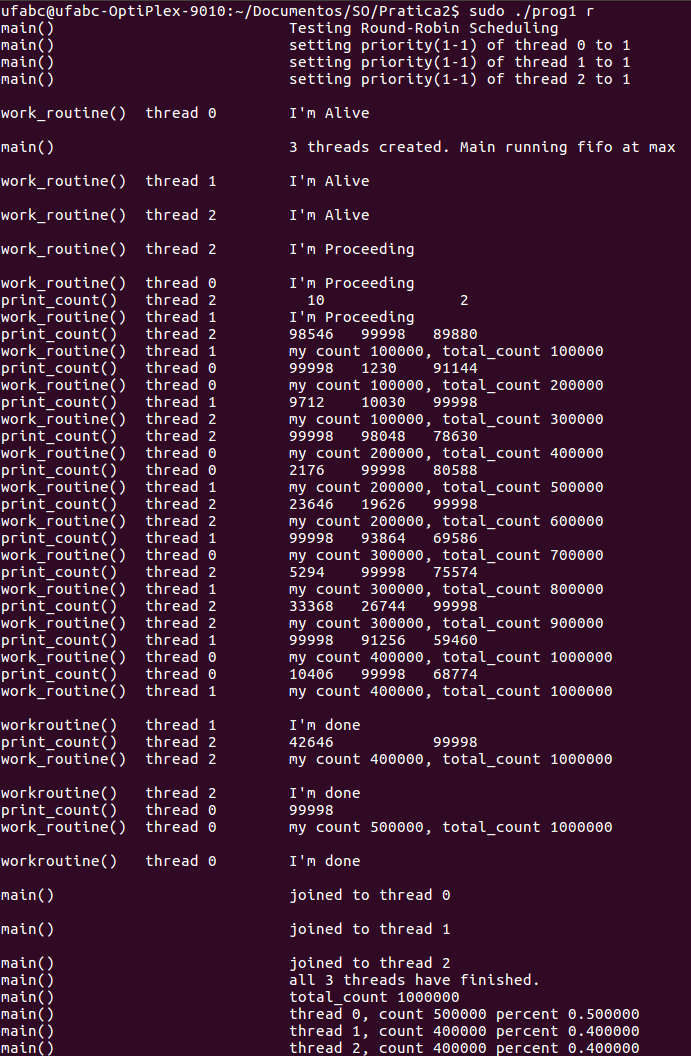
\includegraphics[trim=0 0 0 0,clip,scale=.25]{pratica2/prog1-r.png}
        
        (b)
    \end{minipage}
    \hfill
    \begin{minipage}[b]{0.32\textwidth}
        \centering
        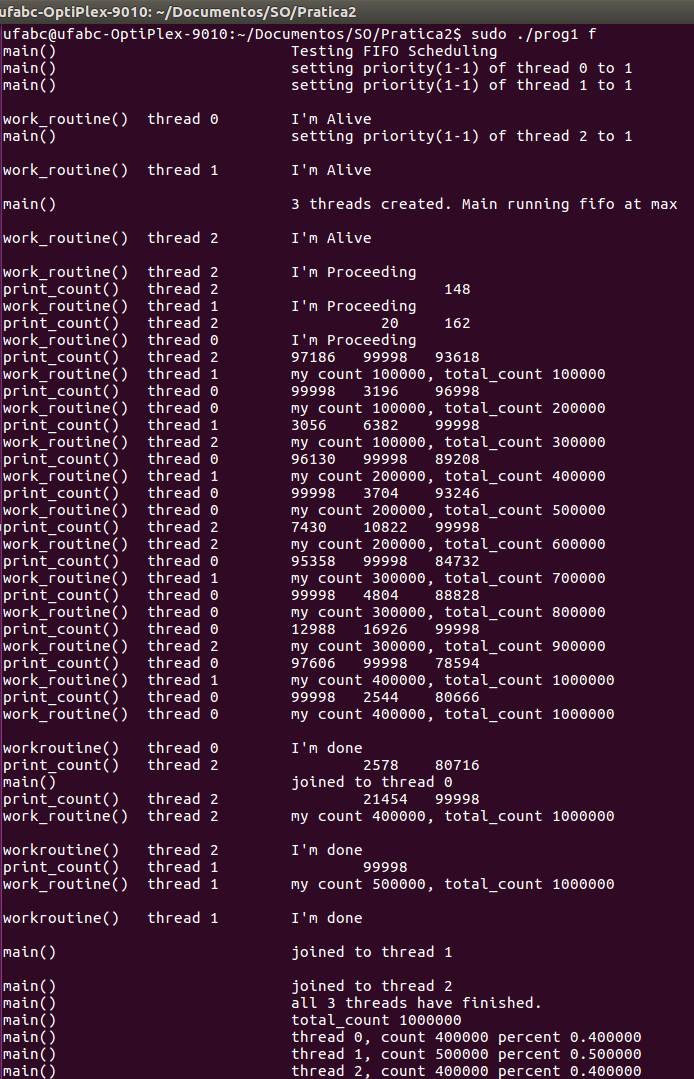
\includegraphics[trim=0 0 0 0,clip,scale=.25]{pratica2/prog1-f.png}
        
        (c)
    \end{minipage}
    \hspace{1em}
    \\
    \hspace{-1em}
    \begin{minipage}[b]{0.32\textwidth}
        \centering
        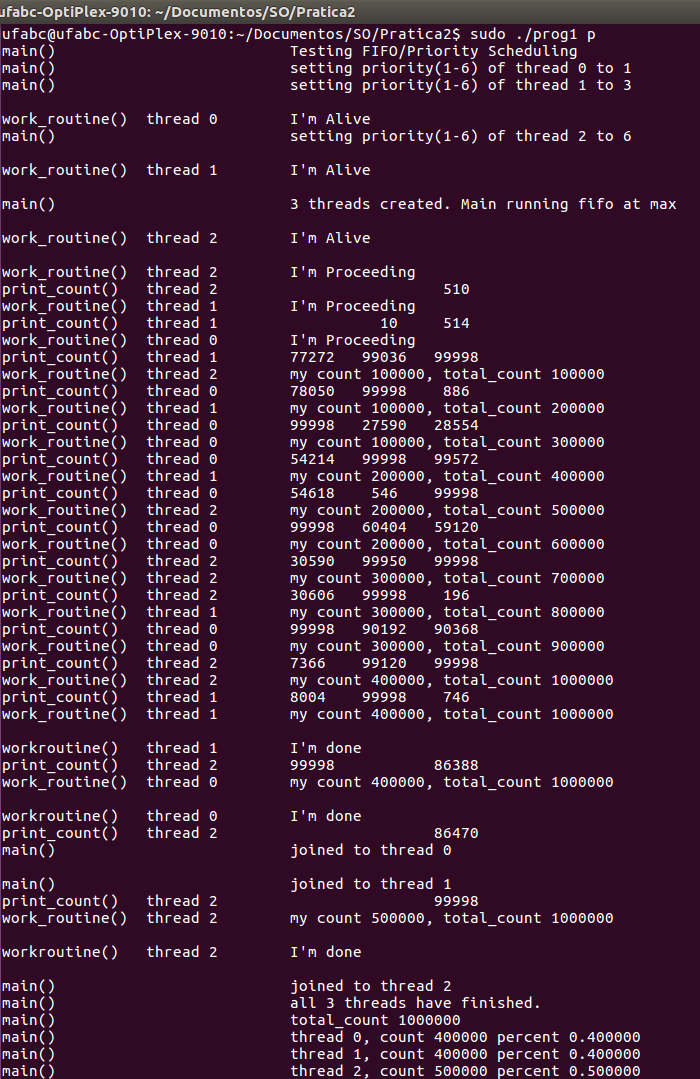
\includegraphics[trim=0 0 0 0,clip,scale=.25]{pratica2/prog1-p.png}
        
        (d)
    \end{minipage}
    \hfill
    \begin{minipage}[b]{0.32\textwidth}
        \centering
        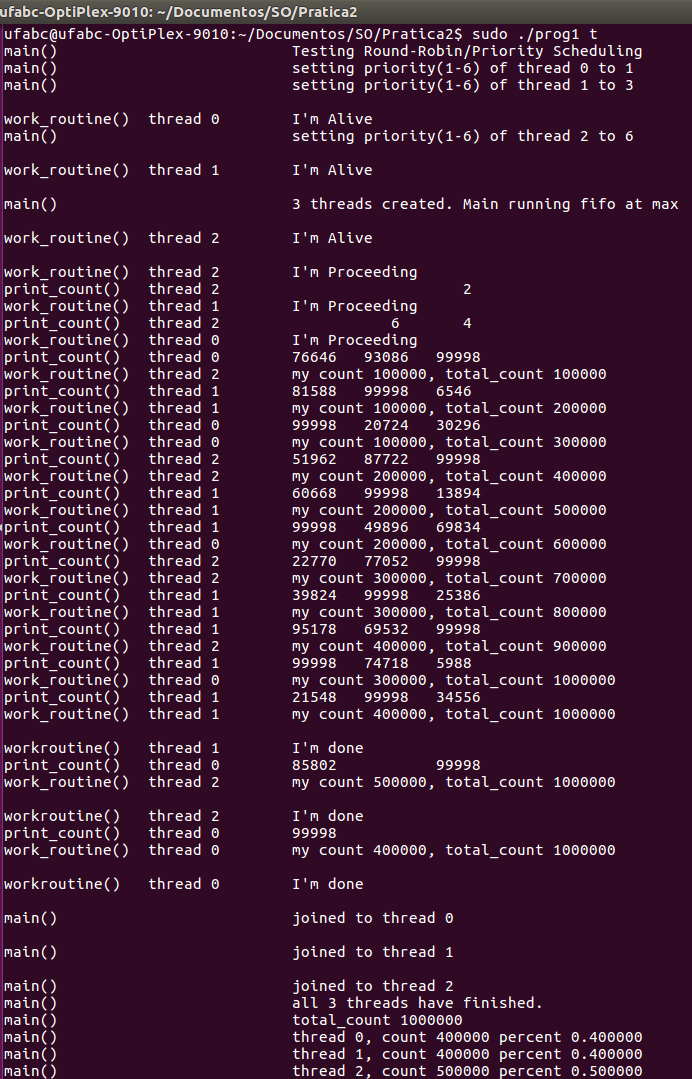
\includegraphics[trim=0 0 0 0,clip,scale=.25]{pratica2/prog1-t.png}
        
        (e)
    \end{minipage}
    \hfill
    \begin{minipage}[b]{0.32\textwidth}
        \centering
        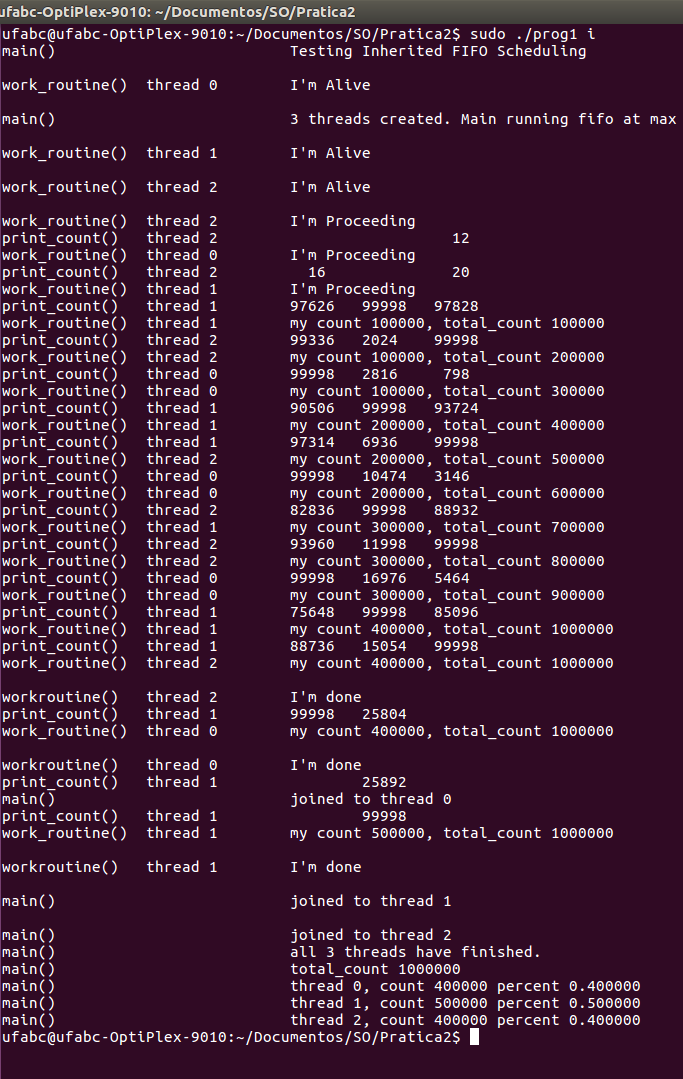
\includegraphics[trim=0 0 0 0,clip,scale=.25]{pratica2/prog1-i.png}
        
        (f)
    \end{minipage}
    \hspace{1em}
    \\[6pt]
    \hspace{-1em}
    \begin{minipage}{\textwidth}
        \centering
        \captionof{figure}{Execução do prog1.c com diferentes parâmetros}
        \label{prog4modpng}
    \end{minipage}
    \hfill
\end{minipage}
\vspace{1em}

\subsection*{2. Uso de variáveis de condição}
\addcontentsline{toc}{section}{2. Uso de variáveis de condição}

\subsubsection{2.1 - Compile com a opção -pthread e execute o programa prog2.c. Explique o uso das variáveis de condição no código do programa.}
\addcontentsline{toc}{subsection}{Exercício 2.1}

\vspace{-0.5em}
\begin{minipage}{\textwidth}
  \hspace{-1em}
  \centering
  \lstinputlisting[language=C]{pratica2/prog2.c}
  \captionof{figure}{Código fonte do programa prog2.c}
  \label{prog4mod}
  \hspace{1em}
\end{minipage}
\vspace{0.5em}

O método \textbf{pthread{\_}mutex{\_}lock (\&\textit{mutex})}, nas linhas 39 e 61, tentam adquirir a trava do \textit{\textbf{mutex}}, colocando a thread em espera até que consiga.

O método \textbf{pthread{\_}cond{\_}wait (\&\textit{cond} , \&\textit{mutex})}, nas linhas 45 e 67, travam a variável \textit{\textbf{cond}} e soltam a trava do \textit{\textbf{mutex}}, e então tenta imediatamente readquirir a trava do \textit{\textbf{mutex}} assim que a variável \textit{\textbf{cond}} permitir, o que faz a thread entrar em espera.

O método \textbf{pthread{\_}cond{\_}signal (\&\textit{cond})}, nas linhas 50 e 72, soltam a trava da variável \textit{\textbf{cond}}, o que não faz a thread esperando no método anterior instantaneamente destravar, pois ela ainda não pode readquirir a trava do \textit{\textbf{mutex}}.

Por fim, o método \textbf{pthread{\_}mutex{\_}unlock (\&\textit{mutex})}, nas linhas 51 e 73, soltam a trava do \textit{\textbf{mutex}}, permitindo que o método \textbf{pthread{\_}cond{\_}wait} o aquira caso possa ou que o método \textbf{pthread{\_}mutex{\_}lock} o recupere na próxima interação do laço.

O uso dessa variável condicional permite, para além da função do semáfaro mutex de proteger regiões críticas, sincronizar as diferentes threads. Utilizando o exemplo desse programa, com a condicional, uma thread não avança quando não há tarefas para realizar ainda.


\vspace{2em}
\begin{minipage}{\textwidth}
    \hspace{-1em}
    \centering
    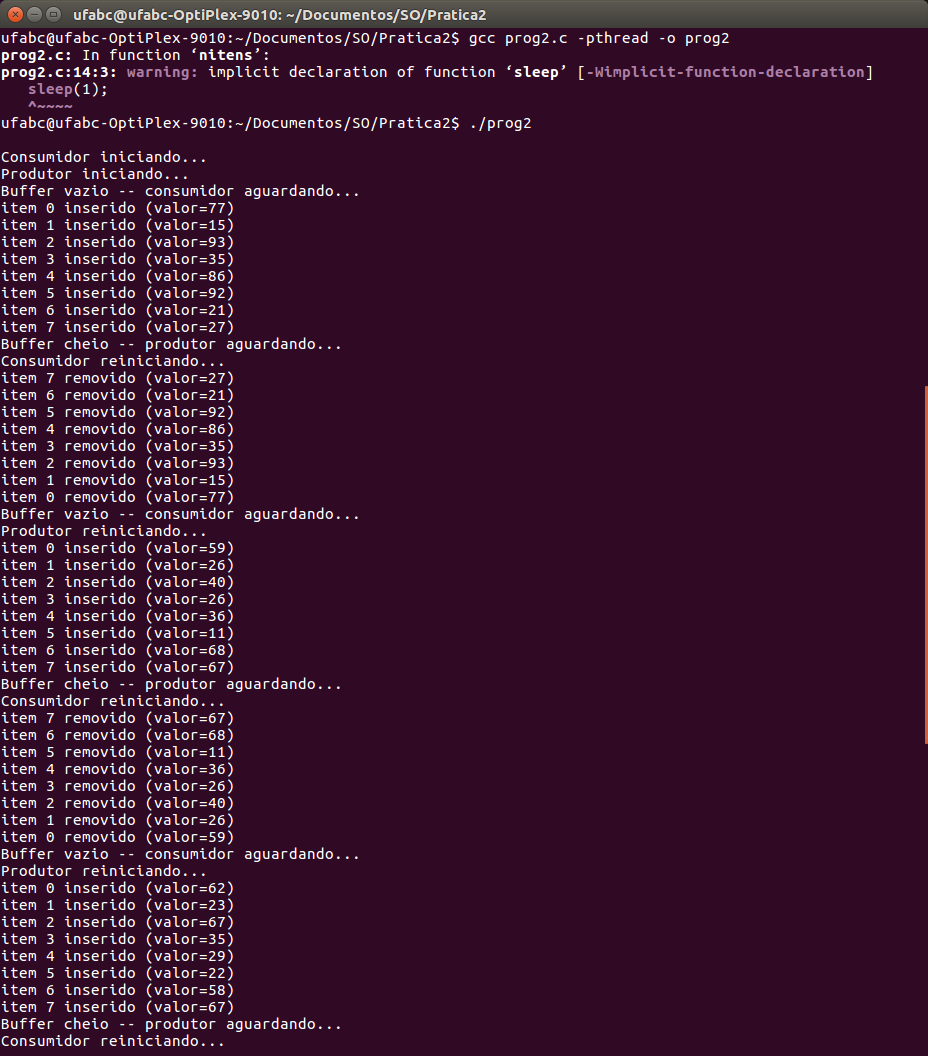
\includegraphics[trim=0 0 0 0,clip,scale=.4]{pratica2/prog2.png}
    \captionof{figure}{Execução do código prog2.c}
    \label{prog4modpng}
    \hspace{1em}
\end{minipage}

\subsection*{3. Impasse}
\addcontentsline{toc}{section}{3. Impasse}

\subsubsection{3.1 - Compile com a opção -pthread e execute o programa prog3.c. O que aconteceu na saída? Justifique.}
\addcontentsline{toc}{subsection}{Exercício 3.1}

Assim que todos os filósofos pegam o primeiro garfo, o programa entra em impasse pois todas as threads estão esperando por um garfo que nunca estará disponível.

\vspace{2em}
\begin{minipage}{\textwidth}
    \hspace{-1em}
    \centering
    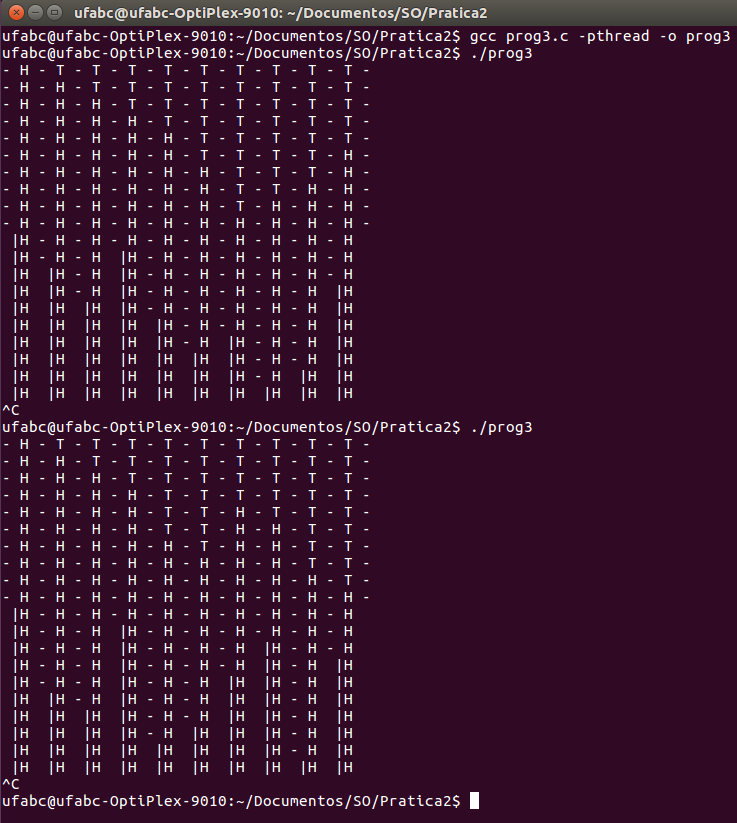
\includegraphics[trim=0 0 0 0,clip,scale=.4]{pratica2/prog3.png}
    \captionof{figure}{Execução do código prog3.c}
    \label{prog4modpng}
    \hspace{1em}
\end{minipage}

\subsubsection{3.2 - Compile com a opção -pthread e execute o programa prog4.c, que é baseado na figura 2.38 do livro texto. O problema do programa anterior foi resolvido? Justifique.}
\addcontentsline{toc}{subsection}{Exercício 3.2}

Foi resolvido, mas às custas do paralelismo da solução, fazendo-o muito lento, já que cada thread tem que esperar as outras terminarem seus ciclos.

\vspace{2em}
\begin{minipage}{\textwidth}
    \hspace{-1em}
    \centering
    \begin{minipage}[b]{0.49\textwidth}
        \centering
        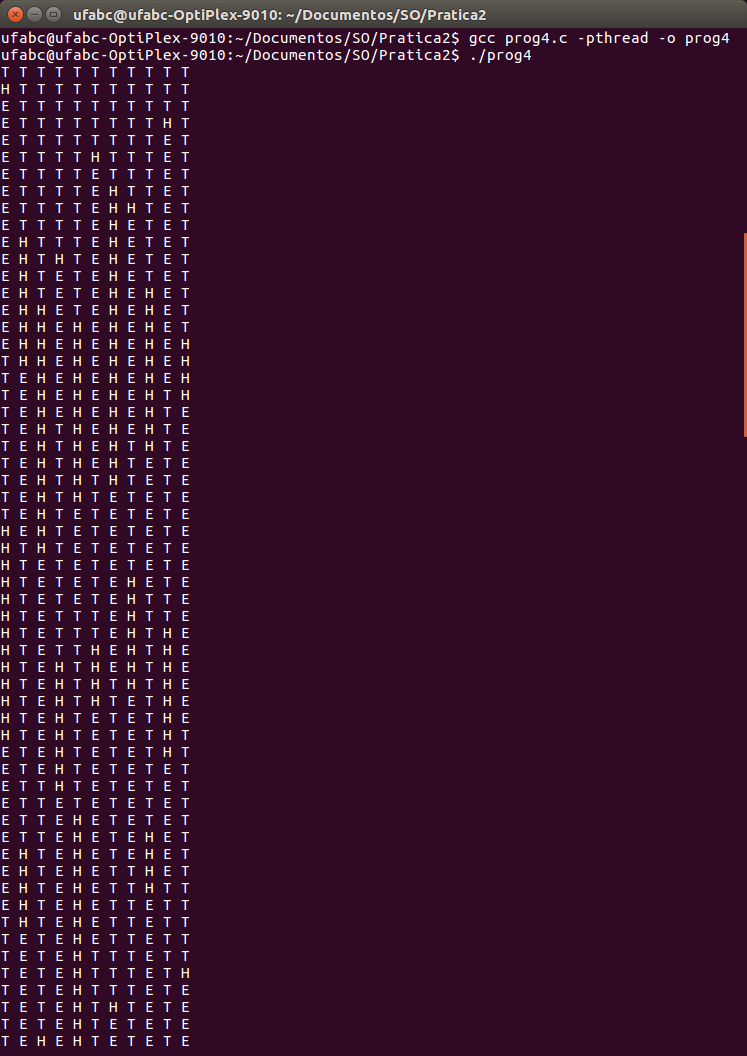
\includegraphics[scale=.3]{pratica2/prog4.png}
        \captionof{figure}{Início da execução do código prog4.c}
        \label{prog5kill1png}
    \end{minipage}
    \hfill
    \begin{minipage}[b]{0.49\textwidth}
        \centering
        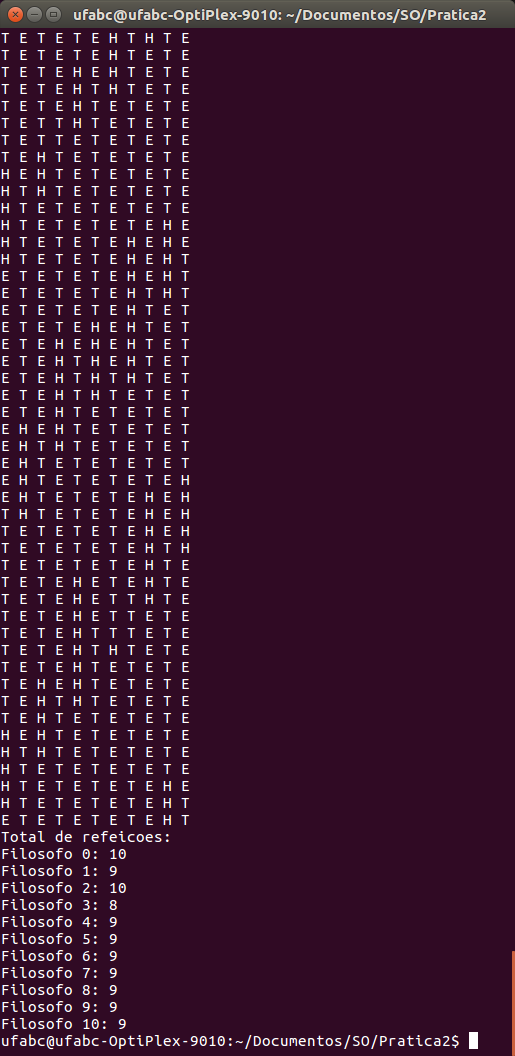
\includegraphics[scale=.3]{pratica2/prog4cont.png}
        \captionof{figure}{Término da execução do código prog4.c}
        \label{prog5kill2png}
    \end{minipage}
    \hspace{1em}
\end{minipage}

\subsection*{4. Inanição (starvation) e desempenho}
\addcontentsline{toc}{section}{4. Inanição (starvation) e desempenho}

\subsubsection{4.1 - Compile com a opção -pthread e execute o programa prog5.c. O que aconteceu na saída? Justifique.}
\addcontentsline{toc}{subsection}{Exercício 4.1}

Ocorre inanição pois cada thread escritor espera as threads leitor terminarem todo seu trabalho antes de começar, e ainda assim somente uma thread opera por vez, ficando assim demasiadamente ociosas.

\vspace{2em}
\begin{minipage}{\textwidth}
    \hspace{-1em}
    \centering
    \begin{minipage}[b]{0.49\textwidth}
        \centering
        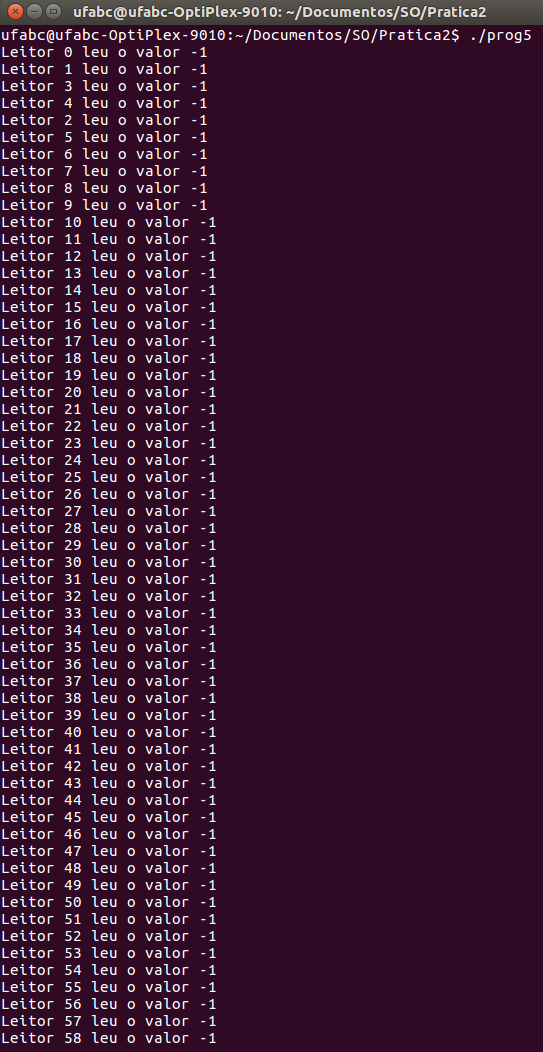
\includegraphics[scale=.3]{pratica2/prog5.png}
        \captionof{figure}{Início da execução do código prog5.c}
        \label{prog5kill1png}
    \end{minipage}
    \hfill
    \begin{minipage}[b]{0.49\textwidth}
        \centering
        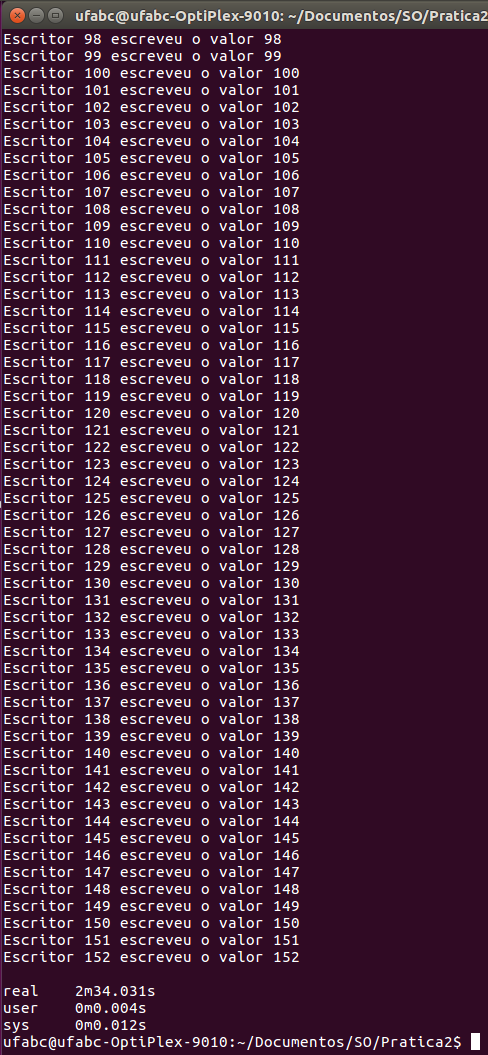
\includegraphics[scale=.3]{pratica2/time-prog5.png}
        \captionof{figure}{Término da execução do código prog5.c}
        \label{prog5kill2png}
    \end{minipage}
    \hspace{1em}
\end{minipage}

\subsubsection{4.2 - Compile com a opção -pthread e execute o programa prog6.c. O problema do programa anterior foi resolvido? Há espaço para melhoria de desempenho da leitura no código?}
\addcontentsline{toc}{subsection}{Exercício 4.2}

Sim, agora as threads escritor e leitor se intercalam (não-deterministicamente) por meio do semáfaro, pois somente um leitor pode ler por vez, passando a vez para outro leitor ou para um escritor. Deve haver uma maneira de permitir leitura simultânea sem causar inanição.

\vspace{2em}
\begin{minipage}{\textwidth}
    \hspace{-1em}
    \centering
    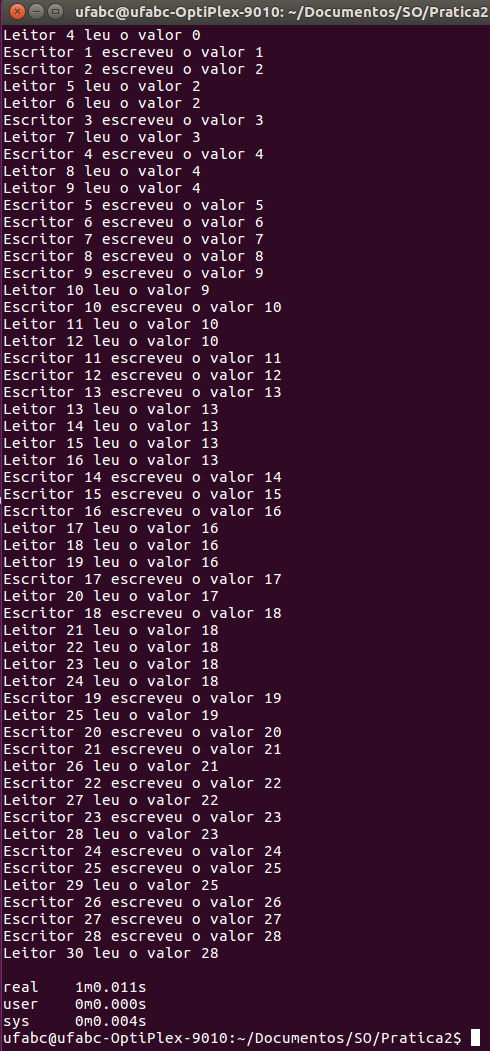
\includegraphics[trim=0 0 0 0,clip,scale=.4]{pratica2/time-prog6.png}
        \captionof{figure}{Término da execução do código prog6.c}
    \label{prog4modpng}
    \hspace{1em}
\end{minipage}

\subsubsection{4.3 - Compile com a opção -pthread e execute o programa prog7.c. Houve melhoria de desempenho na leitura em relação ao programa anterior? Justifique.}
\addcontentsline{toc}{subsection}{Exercício 4.3}

Sim, pois trocando semáfaros por variáveis condicionais agora é possível que vários leitores iniciem a leitura ao mesmo tempo, mas quando um escritor solicitar escrita, nenhum novo leitor pode iniciar a leitura, e quando todos os leitores atuais terminarem de ler, o escritor escreve e devolve aos leitores o poder de iniciar leitura, assim há intercalamento de escritores e leitores, mas também leitura simultânea.

\vspace{2em}
\begin{minipage}{\textwidth}
    \hspace{-1em}
    \centering
    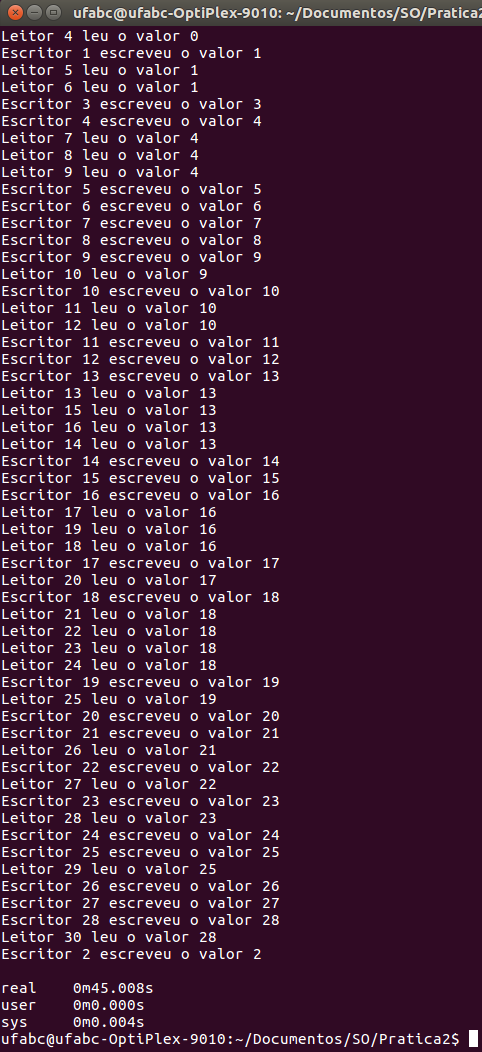
\includegraphics[trim=0 0 0 0,clip,scale=.4]{pratica2/time-prog7.png}
        \captionof{figure}{Término da execução do código prog7.c}
    \label{prog4modpng}
    \hspace{1em}
\end{minipage}